\section{Analysis}\label{sec:analysis}

Sonar Workbench includes built-in functions to assist with analysis.  Version 1.0 concentrates on array building, conventional beam pattern synthesis, and beam pattern analysis. Planned upgrades include support for adaptive beamforming, element and array radiation impedance, and array gain in anisotropic noise.

\subsection{Plotting arrays}

The function \texttt{PlotArray.m} creates a 3D plot of an array. Usage instructions are shown in Listing~\ref{lst:PlotArray}.

\lstinputlisting[firstline=2,lastline=36,caption={\texttt{PlotArray.m}},label={lst:PlotArray}]{../../mdl/PlotArray.m}
 
The user must pass the array and element structures as the first two parameters to \texttt{PlotArray.m}. This will produce a physical plot of the array, as shown in \figname~\ref{fig:SampleArray}. There are three optional inputs to \texttt{PlotArray.m}. The user can enter empty brackets \texttt{[]} for any optional parameters that are not needed. If the user inputs a beam structure in the third parameter, the elements will be filled with a solid color whose opacity is proportional to the amplitude weights, as shown in \figname~\ref{fig:SampleBeam}. To plot the array in an existing figure axis, pass a handle to that axis as the fourth parameter, \texttt{hax}. The Matlab function \texttt{gca} can be used to specify the current axis. The fifth parameter lets the user plot the array scaled to dimensions of 1 unit = 1 meter. This is helpful if the array is to be overlaid on a user-generated plot of its host platform. 
 
\subsection{Calculating beam patterns}

\texttt{BeamPattern.m} calculates the beam pattern for wavelength $\lambda$, elevation angles $\theta$, and azimuthal angles $\psi$ as
\begin{equation}
BP(\lambda,\theta,\psi) = \sum_{i=1}^{N_e} w_i(\lambda,\theta_0,\psi_0)E_i(\lambda,\theta,\psi)e^{j2\pi\left(\frac{\cos\theta\cos\psi}{\lambda}x_i + \frac{\cos\theta\sin\psi}{\lambda}y_i + \frac{\sin\theta}{\lambda}z_i\right)},
\end{equation}
where, for the $i^{th}$ element in the array, $w_i(\lambda,\theta_0,\psi_0)$ is the complex weight, $E_i(\lambda,\theta,\psi)$ is the element pattern, rotated according to the element orientation ($\gamma_i$,$\theta_i$,$\psi_i$), and ($x_i$,$y_i$,$z_i$) are the element coordinates. This computation is performed in the array frame. The resulting beam pattern can be converted to the body frame through an appropriate translation and rotation.

The beam pattern is returned in complex linear units. This retains the amplitude and phase information from the beam. The amplitude is normalized by dividing the output by the sum of the beam weight amplitudes,
\begin{equation}
BP_{norm}(\lambda,\theta,\psi) = \frac{BP(\lambda,\theta,\psi)}{\sum_{i=1}^{N_e}|w_i(\lambda,\theta_0,\psi_0)|}.
\end{equation}
For an unsteered beam, this produces an output with amplitude 1 along the maximum response axis. Steering beams off axis can result in a peak beam amplitude less than 1.

Usage instructions for \texttt{BeamPattern.m} are shown in Listing~\ref{lst:BeamPattern}. All input parameters are required. The first three are the array, element, and beam structures. The fourth parameter is the wavelength, $\lambda$. This must be a scalar. 

The final two parameters are the elevation and azimuthal angles over which the beam pattern is to be calculated, in degrees. These parameters can be scalars, vectors, or matrices, but they must have compatible dimensions. If both are scalars, the output, \texttt{BP}, will be a scalar. If both are vectors, \texttt{BeamPattern.m} uses the Matlab function \texttt{ndgrid} to calculate a matrix \texttt{BP}, with rows corresponding to $\theta$ and columns corresponding to $\psi$. The user can generate their own matrix inputs using \texttt{[Theta,Psi] = ndgrid(theta,psi);} for vectors \texttt{theta} and \texttt{psi}.

\lstinputlisting[firstline=2,lastline=49,caption={\texttt{BeamPattern.m}},label={lst:BeamPattern}]{../../mdl/BeamPattern.m}

\subsection{Plotting beam patterns}

The function \texttt{Plot3DBP.m} plots the three dimensional beam magnitude with decibel scaling. Usage instructions are shown in Listing~\ref{lst:Plot3DBP}. The three required inputs are elevation and azimuthal angle vectors, $\theta$ and $\psi$ in degrees, and the beam pattern matrix. 

The first optional input, \texttt{PlotType}, selects a plot with the beam pattern surface and color proportional to magnitude when its value is 1, and it selects a pot with the beam pattern color proportional to magnitude but drawn on a surface of constant radius when its value is 2. Examples of these two options are shown in the left and right panels of \figname~\ref{fig:SampleBeam} Those plots are for the example element, array, and beam defined in Listings~\ref{lst:SampleElement}, \ref{lst:SampleArray}, and \ref{lst:SampleBeam}.

The second optional input, \texttt{dBScale}, is a two-element vector with the minimum and maximum magnitudes in dB. The default values are -40 and 0 dB. It is common to use 0 dB for the maximum value, since the beam pattern is normalized by default.

The third optional input is the axis handle, \texttt{hax}, in which to plot the beam. This input has the same functionality as it does in \texttt{PlotArray.m}, and it allows the beam to be plotted with the array on the same axis. Matlab function \texttt{gca} can be used to specify the current axis.

The final optional inputs allow the beam to be offset according to the array position in the body frame. 

\lstinputlisting[firstline=2,lastline=26,caption={\texttt{Plot3DBP.m}},label={lst:Plot3DBP}]{../../mdl/Plot3DBP.m}

\clearpage
\begin{sidewaysfigure}[!ht]
\begin{center}
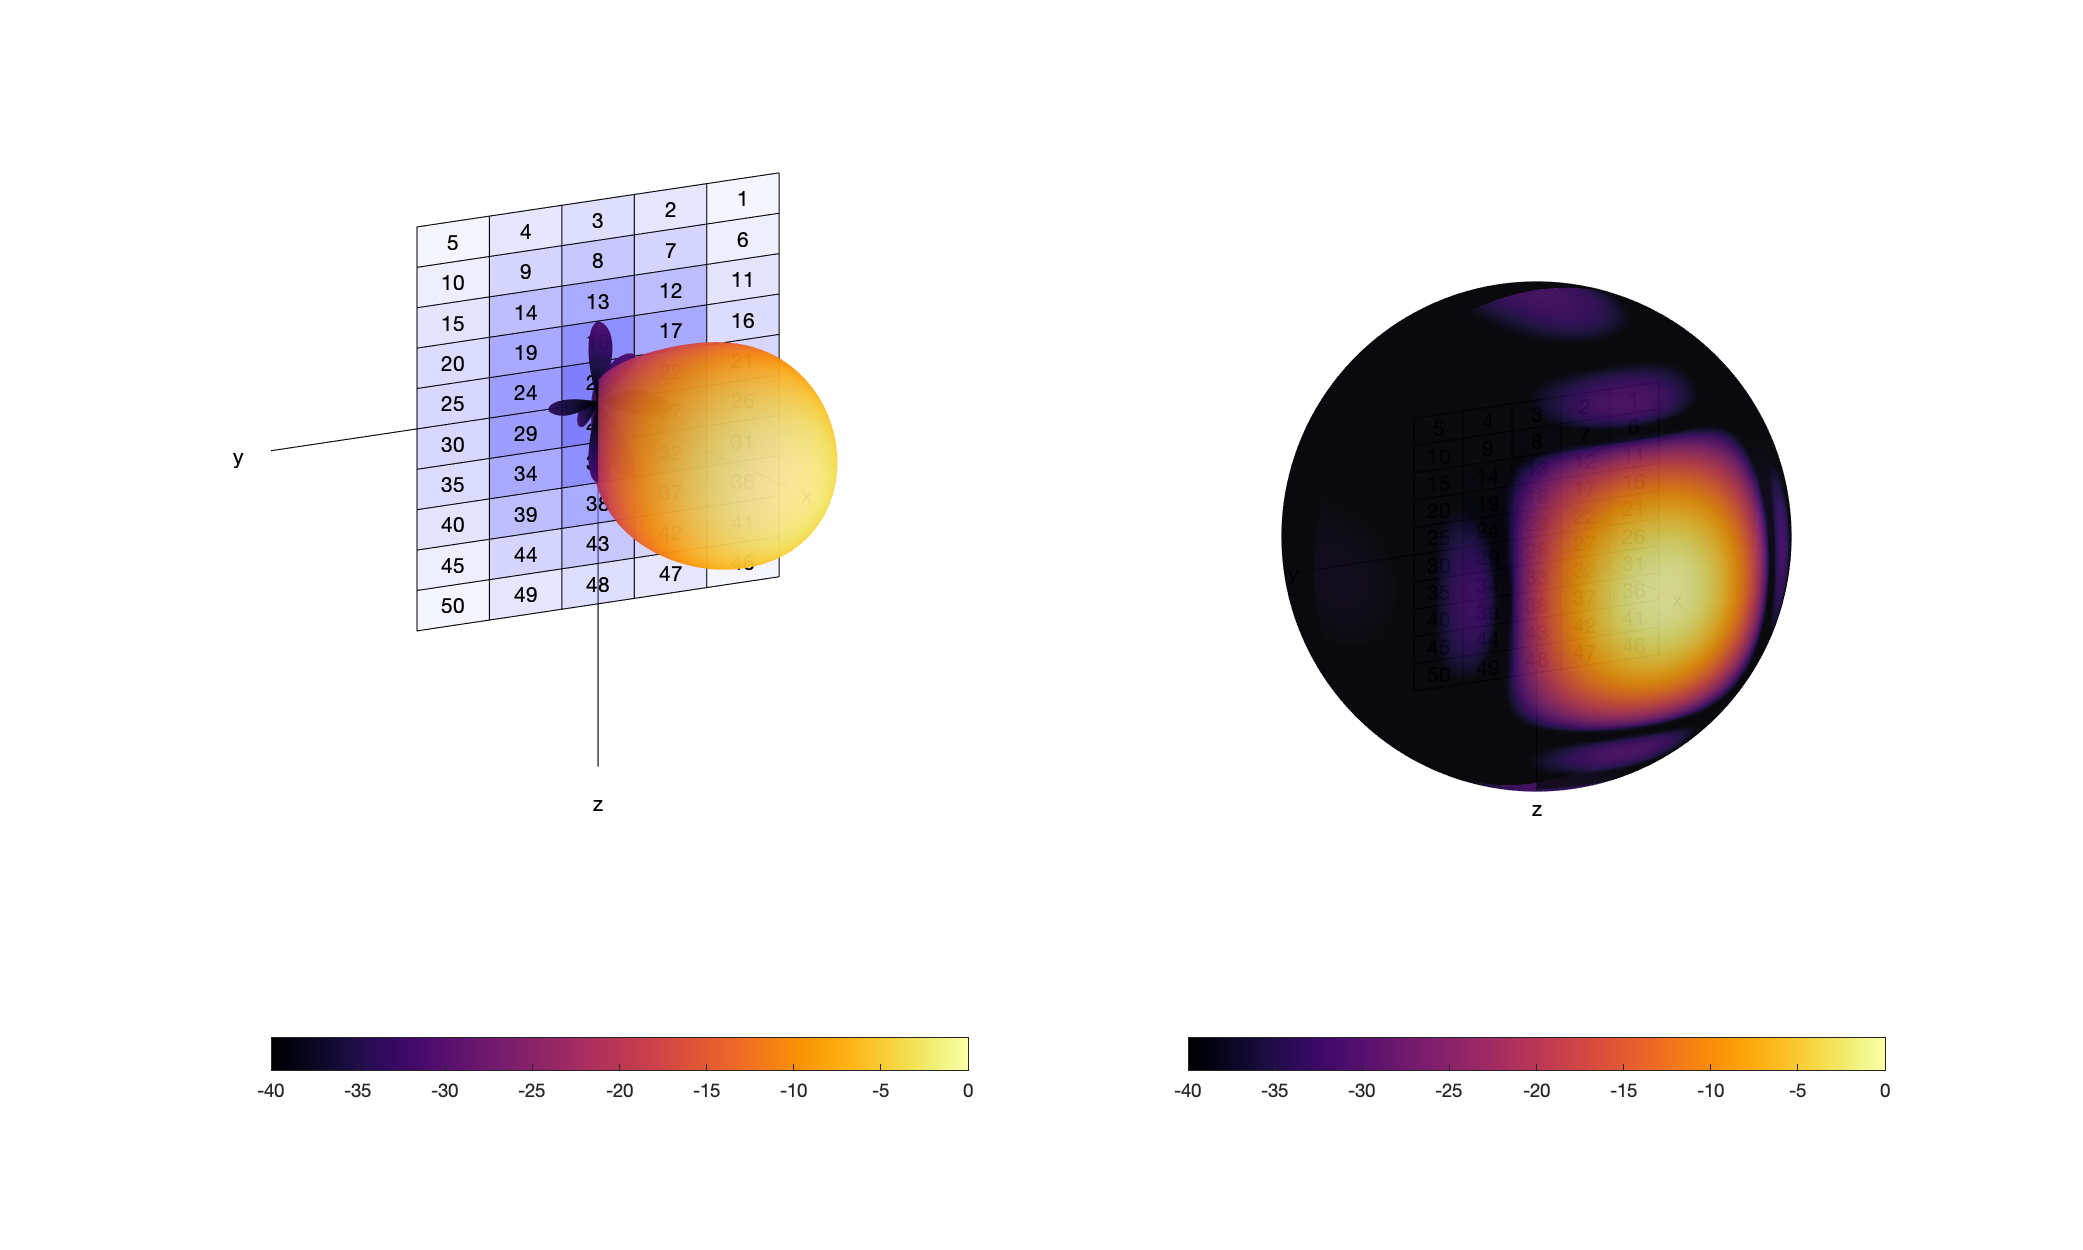
\includegraphics[width=8in]{SampleBeam}
\caption{\label{fig:SampleBeam}Example beam pattern for rectangular planar array}
\end{center}
\end{sidewaysfigure}

\clearpage
\subsection{Calculating beam width}

Beam width is the angular span over which the beam magnitude is within 3 dB of its peak value. Sonar Workbench contains two functions to calculate beam width: \texttt{BeamWidth.m} for 2D beams, which computes beam width in a single plane, and \texttt{BeamWidth3D.m} for 3D beams, which computes vertical and horizontal beam widths. Usage is shown in Listings~\ref{lst:BeamWidth} and \ref{lst:BeamWidth3D}.

\lstinputlisting[firstline=2,lastline=20,caption={\texttt{BeamWidth.m}},label={lst:BeamWidth}]{../../mdl/BeamWidth.m}

\lstinputlisting[firstline=2,lastline=25,caption={\texttt{BeamWidth3D.m}},label={lst:BeamWidth3D}]{../../mdl/BeamWidth3D.m}

There are two required parameters for \texttt{BeamWidth.m}. The first, \texttt{ang}, is a vector of angles in degrees over which the beam pattern slice is defined, and the second, \texttt{bp}, is the beam pattern at those angles, in linear units. The user can assist the function in locating the correct peak value to search around by specifying an approximate peak angle in the first optional parameter, \texttt{ang0}. The final optional parameter, \texttt{renorm}, instructs the function to re-normalize the beam pattern to have a peak magnitude of 0 dB before searching for the -3 dB angles. This can be useful for a steered beam whose peak magnitude is less than 0 dB. 

The output, \texttt{BW}, is the measured beam width in degrees. The function attempts to interpolate between input grid angles using spline interpolation of the beam magnitude in dB. The user can get a more precise measurement by using finer angle sampling. If \texttt{BeamWidth.m} can not calculate a valid beam width, it returns \texttt{NaN}.

\texttt{BeamWidth3D} has similar usage but with expanded support for an additional dimension. Its first three parameters are required, and correspond to angle vectors $\theta$ and $\psi$ in degrees and beam pattern matrix \texttt{BP} in linear units. The first two optional parameters, \texttt{theta0} and \texttt{psi0} serve the same purpose as \texttt{ang0} in \texttt{BeamWidth.m} for the elevation and azimuthal angles, respectively. The final optional parameter, \texttt{renorm}, is identical to that parameter in \texttt{BeamWidth.m}. There are two outputs, \texttt{BWV} and \texttt{BWH}, which are the vertical and horizontal beam widths in degrees, respectively. For the example beam in \figname~\ref{fig:SampleBeam}, the vertical and horizontal beam widths are calculated to be 26$^\circ$ and 25.6$^\circ$.

\subsection{Calculating directivity index}

Directivity Index (DI) is a measure of a beam's ability to filter spatially isotropic noise. It is the ratio of the noise level received by an omnidirectional sensor to the noise level received by the beam, expressed in dB. It is calculated from the Directivity (D) according to
\begin{equation}
DI(\lambda) = 10\log_{10}D(\lambda),\label{eq:DirectivityIndex}
\end{equation}
where
\begin{equation}
D(\lambda) = \frac{4\pi}{\int_0^{\pi}\int_0^{2\pi}|BP(\lambda,\theta,\psi)|^2d\psi{d\theta}}.\label{eq:Directivity}
\end{equation}

\texttt{CalculateDI.m} implements \eqnnames~(\ref{eq:DirectivityIndex}) and (\ref{eq:Directivity}) using numerical integration over a realized beam pattern. Usage is shown in Listing~\ref{lst:CalculateDI}.

There are three required parameters. The first two are angle vectors $\theta$ and $\psi$ in degrees, and the third is the beam pattern matrix \texttt{BP} in linear units. For best results, $\theta$ should span 180$^\circ$ vertically, and $\psi$ should span 360$^\circ$ horizontally. If instead, the beam pattern is defined as a subset of these angles, \texttt{CalculateDI.m} assumes the beam pattern value is exactly zero outside the defined region. There is a single output, \texttt{DI}, which is the directivity index in dB.

\lstinputlisting[firstline=2,lastline=17,caption={\texttt{CalculateDI.m}},label={lst:CalculateDI}]{../../mdl/CalculateDI.m}